\section{Experiments: both accounts, scored}
\label{sec:evidence}

This section scores both accounts of \S\ref{sec:theory} against one
measured object: debiased demotion-gap curves over the full $\sigma$
axis, on routes neither account saw. We build the instrument
(\S\ref{sec:instrument}); read the per-route map its curves certify
--- the deployed artifact (\S\ref{sec:map}); then score both accounts
against the same curves --- the spectral one at the boundary and the
curve level, ours term by term (\S\ref{sec:scored}). The held-out
prediction protocol, its pre-registered gates, and the structural
failures it exposes are quantified in
Appendix~\ref{sec:headtohead}. Each subsection states
the prediction it discharges against criteria frozen before the runs;
several probes double as falsifiers of our own account's assumptions.

\subsection{The instrument}
\label{sec:instrument}

\paragraph{Model and data.}
All measurements use Anima \citep{circlestone2025anima}, an open
DiT-based flow-matching text-to-image model (2B parameters, 28
transformer blocks, 3D rotary position embeddings, and the Qwen-Image
VAE, \citealp{wu2025qwenimage}), fine-tuned with LoRA adapters on an
illustration corpus. Images are bucketed by native aspect ratio into
resolution \emph{tiers} indexed by nominal edge length
$e \in \{512, 768, 896, 1024, 1280\}$; a tier-$e$ image occupies roughly
$(e/16)^2$ latent-patch tokens (${\sim}4{,}100$ at 1024, ${\sim}3{,}000$
at 896, ${\sim}2{,}160$ at 768, ${\sim}1{,}000$ at 512). The probe
adapter is a plain LoRA checkpoint trained at native tiers; we return to
this operating-point dependence in \S\ref{sec:limitations}.

\paragraph{The gradient probe.}
For each image and each of $B$ $\sigma$-bins we accumulate
adapter gradients over $D$ stratified noise draws per
arm\footnote{Finite draws are not innocuous here. Every finite-draw
cosine is attenuated below its population value; the attenuation is
arm-dependent, because per-draw gradient variance grows as the token
count falls (the MSE loss averages over fewer elements); and the
natural estimate of Eq.~\ref{eq:gapdef} --- a redraw floor minus a
single demoted-arm cosine --- is asymmetric, the floor comparing
\emph{two} finite-draw estimates of the native gradient where each
demote arm contributes one. An iso-direction null (demotion changing
\emph{nothing} but the variance) therefore still produces a positive
gap that \emph{grows as the target grid shrinks} --- the same
signature as ``absolute token count sets the floor'' --- and no naive
read can tell the two apart. The mechanism is live and large at our
operating point (measured magnitudes and $c/D$ decay:
Appendix~\ref{app:instrument}).} (verdict
run: $14$ interior bins on a segmented grid dense below $\sigma = 0.1$
and above $0.9$, plus a $\sigma{=}1$ endpoint bin, $D{=}12$,
deterministic kernels; $N = 40$ images) and compare arms by cosine
similarity of the flattened accumulated gradients: a \textbf{floor}
(two independent draw sets at native resolution, the redraw null); the
\textbf{reenc} control of \S\ref{sec:estimand}; one \textbf{demote} arm
per edge $e$; and, on debiased runs, per-arm \textbf{self-floors} (a
second independent draw set for every arm). The gap is in cosine units,
a scale-free mismatch \emph{fraction} (bin-mean SEM $0.01$--$0.07$ at
$N{=}40$). Gap subtraction, not absolute cosines, is the valid read:
the floor itself moves with $\|g\|$ across bins. Every bin-mean curve
must pass a split-half reliability check over images, a discipline
imposed after an earlier failure in which per-image rankings from the
same gradients had reliability indistinguishable from zero.

\paragraph{The debiased estimator.}
Two corrections, used together, remove the finite-draw attenuation.
First, \emph{self-floors with
attenuation correction}: every arm runs a second independent draw set
$g_a'$, giving a per-arm self-cosine
$\cos_{\mathrm{self}} = \cos(g_a, g_a')$, so that each arm has the same
two-estimate structure the native floor has. The debiased cosine is the
classical split-half disattenuation correction,
\begin{equation}
\hat c \;=\; \frac{\cos(\bar g_{\src},\, \bar g_{a})}
{\sqrt{\cos_{\mathrm{floor}} \cdot \cos_{\mathrm{self},a}}},
\qquad
\dgap \;=\; 1 - \hat c,
\label{eq:debias}
\end{equation}
which cancels the finite-draw attenuation of numerator and denominator
to first order. Second, \emph{draw-count extrapolation}: the attenuation
of an accumulated-draw cosine decays as $1/D$, so sweeping nested draw
subsets and fitting $\gap(D) = \gap_\infty + c/D$ reads off the
draw-limit gap directly. The two are mutually checking, and the check
passes: debiased fits come out $D$-flat, and the nested sweep
extrapolates the native redraw floor to a self-cosine of
${\approx}\,1$ --- the population per-bin native gradient is a
\emph{fixed direction}, and the entire redraw floor is finite-draw
noise (validation numbers: Appendix~\ref{app:instrument}). No
conclusion in this paper survives on the naive estimator alone.

\paragraph{Margins and resolution.}
Any estimate of $\gap_e(\sigma)$ compares finite-draw estimates of
population directions, so a safety verdict needs two numbers, and they
must be stated \emph{separately}: a margin --- the largest excess
considered practically equivalent, a property of the question --- and
the instrument's resolution, which determines only the power available
to certify that margin. Conflating them would let a noisier experiment
buy itself a looser definition of safety. We fix the practical margin
at $\varepsilon = 0.02$, comparable to the re-encode control's own
confidence half-width (Table~\ref{tab:floor}), independent of $N$,
$D$, and the observed standard errors. A route is \emph{certified safe
at margin $\varepsilon$} in a bin exactly where the one-sided
non-inferiority bound clears it,
\begin{equation}
\text{UB}_{95}\!\left(\bgap\right) \;<\; \varepsilon,
\label{eq:safe}
\end{equation}
and a \emph{window} claim over several bins requires the simultaneous
(Bonferroni-corrected) one-sided bounds to clear it in every bin.
Resolution enters only through power: for a route whose true excess is
zero the paired estimate $\bgap$ fluctuates with standard error
$\mathrm{SE}(N, D, \sigma\text{-bin})$, and its zero-excess upper
bound $\epsstar(N, D, \text{bin}) = 1.645\,\mathrm{SE}$ is the
\emph{certification resolution}. A cell with $\epsstar > \varepsilon$
is \emph{underpowered} at the margin: a crossing there can occur on a
favorable draw and is reported but not counted as certification, and
the remedy is more images or draws, never a looser margin. ``No
certifiable window'' means a route's simultaneous upper bounds do not
cross below $\varepsilon$ at the current $(N, D)$; ``certifiably
unsafe'' means the corresponding lower bound stays above it. At the
verdict grid's operating point ($N{=}40$, $D{=}12$/bin) the bin-level
$\epsstar$ is $0.02$--$0.07$ --- underpowered at
$\varepsilon = 0.02$, so interior verdicts below are stated as the
margins they \emph{do} certify --- while endpoint-mode draw sweeps
($D$ up to $64$) reach $\epsstar \approx 0.01$--$0.02$ and are powered
for the strict margin. At interior draw counts the \emph{unpaired}
debiased estimator is unstable where the floors are small (mid-$\sigma$; the
denominator is noisy), so all verdict maps report the \emph{paired
per-image excess} $\gap_{e,i} = \dgap_{e,i} - \dgap_{\reenc,i}$,
trimmed of non-finite and $|\gap_{e,i}| > 1.5$ values; pairing cancels
the shared per-image, per-bin draw structure. Finite-draw cosines are
also compiler-kernel-path sensitive, so all pairings live within one
run. Every number in the main text is debiased; four secondary probes
(the $1280$-tier iso-severity twin, the $896$-tier transfer, the depth
split, and the positional-interpolation intervention) predate the
debiased instrument and are retained only where the strictly positive
bias makes an in-band read conservative, or where a paired same-grid
contrast cancels the bias to first order
(Appendices~\ref{app:instrument},~\ref{app:tables}).

\subsection{The measured $(\text{route}, \sigma)$ map}
\label{sec:verdict}
\label{sec:map}

\begin{figure}[t]
\centering
\begin{subfigure}[t]{0.46\textwidth}
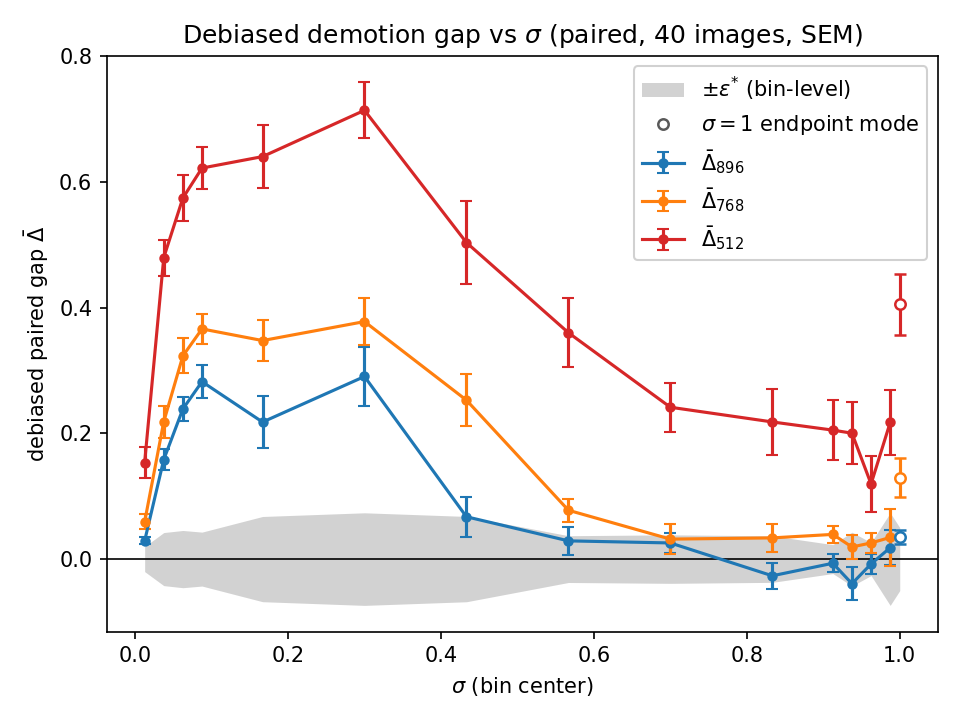
\includegraphics[width=\linewidth]{figs/gap_debiased.png}
\phantomcaption
\label{fig:gapcurves}
\end{subfigure}\hfill
\begin{subfigure}[t]{0.515\textwidth}
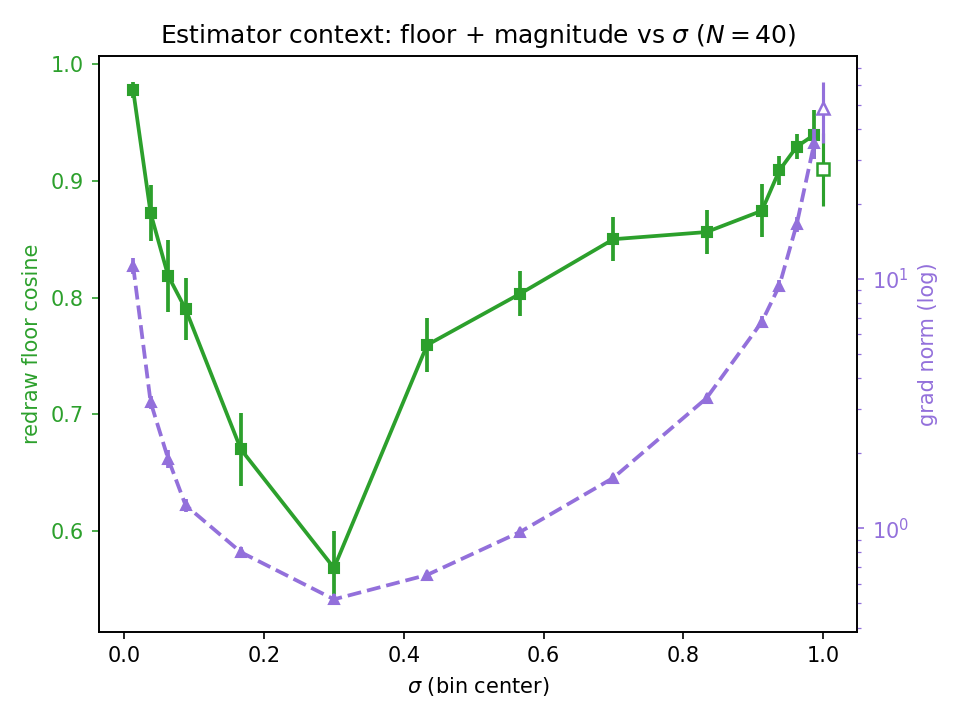
\includegraphics[width=\linewidth]{figs/estimator_context.png}
\phantomcaption
\label{fig:estimator}
\end{subfigure}
\caption{The measurement in detail.
(a)~Debiased demotion gap per $\sigma$-bin, paired against the
re-encoding control ($1024$-tier natives, $N{=}40$; per-bin values and
SEMs in Appendix Table~\ref{tab:debiasedmap}; gray band: bin-level
$\pm\epsstar$ (\S\ref{sec:instrument}); open markers: the $\sigma{=}1$
endpoint bin): safety is a per-route boundary --- the $896$ route
enters the band at $\sigma \approx 0.5$, $768$ falls only to a
low-excess shelf ($+0.02$--$0.04$ over $0.65 < \sigma < 0.95$, short
of the strict margin), and $512$ never falls inside the band (closest
approach $+0.12 \pm 0.05$ at $\sigma = 0.96$) --- against the
spectral family's prediction of $\sigma \approx 0.14$--$0.20$.
(b)~The estimator context those curves are read through: the
redraw-floor cosine and the U-shaped gradient norm
$\|\bar g_{\src}(\sigma)\|$.}
\label{fig:verdict}
\end{figure}

The answer to the title question at our operating point is not a
corrected formula but a measured map at a stated resolution: the
debiased gap curves both accounts are scored on (\S\ref{sec:scored})
carry the verdict, read per bin against the safety statement of
Eq.~\ref{eq:safe} (Fig.~\ref{fig:verdict}; per-bin numbers in Appendix
Table~\ref{tab:debiasedmap}). Collected route by route --- \emph{safe}
meaning Eq.~\ref{eq:safe} holds at the stated margin, on the
\emph{per-example} object --- the map needs no table: $1024{\to}896$
(floor $0.02$--$0.04$) is \textbf{safe} on the interior window
$\sigma \in (0.5, 1)$, certified at margin $0.09$ simultaneous over
the seven window bins ($0.066$ pointwise; the strict
$\varepsilon = 0.02$ margin is not yet powered on the interior grid,
and powering it is a draw-count exercise, designated for the next
probe campaign); $1280{\to}1024$ (floor ${\approx}\,0$) is
\textbf{safe} from $\sigma \gtrsim 0.75$, and the synthetic
iso-severity grid $1280{\to}1120$ is safe with
$\sigmastar \approx 0.5$, as its ratio twin predicts (both
$1280$-tier reads on the pre-debiasing instrument;
\S\ref{sec:limitations}); $1024{\to}768$ and $896{\to}768$ (floors
$0.06$--$0.13$) certify no window at the strict margin, but
$1024{\to}768$ retains a narrow \textbf{low-excess window}
$\sigma \in (0.65, 0.95)$ --- paired excess $+0.02$--$0.04$ per bin,
certified at margin $0.09$ simultaneous over its four window bins
($0.072$ pointwise), atop a floor no noise level removes --- the
window \S\ref{sec:trainer} stacks as a second route; and any route to
$512$ (floor ${\approx}\,0.30$) is \emph{certifiably unsafe} in all
fifteen bins --- no noise level comes near certifying a $2\times$
downscale. Safety is a per-route boundary, jointly determined by
ratio (through $a_e$) and absolute target size (through $\Floor_e$);
neither alone predicts the ordering. Debiasing itself moved verdicts
in both directions, and the two revisions against the historical
record are part of the result: roughly half the $768$ route's
high-$\sigma$ plateau was estimator bias, softening ``unsafe at every
noise level'' into the narrow window just stated, while the $896$
endpoint shows a small \emph{real} gap ($+0.034 \pm 0.011$) that
single-estimate variance had buried --- its safe window is the
interior, not the endpoint (Appendix Table~\ref{tab:rawendpoint}).

\paragraph{A corollary worth stating plainly.}
The safety of $1024{\to}896$ is an \emph{empirical smoothness statement
about this network's function across nearby token counts}, not an
information-theoretic statement about the data. There was no a priori
reason to expect a universal ratio invariant, and the spectral
account's deepest error is having promised one.

\paragraph{The map depends on the aggregation object.}
The aggregation operator is part of the estimand
(\S\ref{sec:estimand}, Appendix~\ref{app:notation}), and the two
objects genuinely disagree at high $\sigma$: pooled-arm probes (pool
size $4$) collapse the $1024{\to}896$ and $1024{\to}768$ excesses to
${\approx}\,0$ over the upper bins --- the batch-aggregate object SGD
follows is more forgiving here than the per-example read we publish
as the verdict. The coherent drift no batch size removes is bounded
only by an $a + b/B$ fit across pool sizes, the designated readout of
a debiased verdict grid at the trainer's actual
batch$\times$accumulation operating point \textbf{[pending]}.

\subsection{Both accounts, scored}
\label{sec:scored}
\label{sec:specscored}
\label{sec:ourscored}

\begin{figure}[t]
\centering
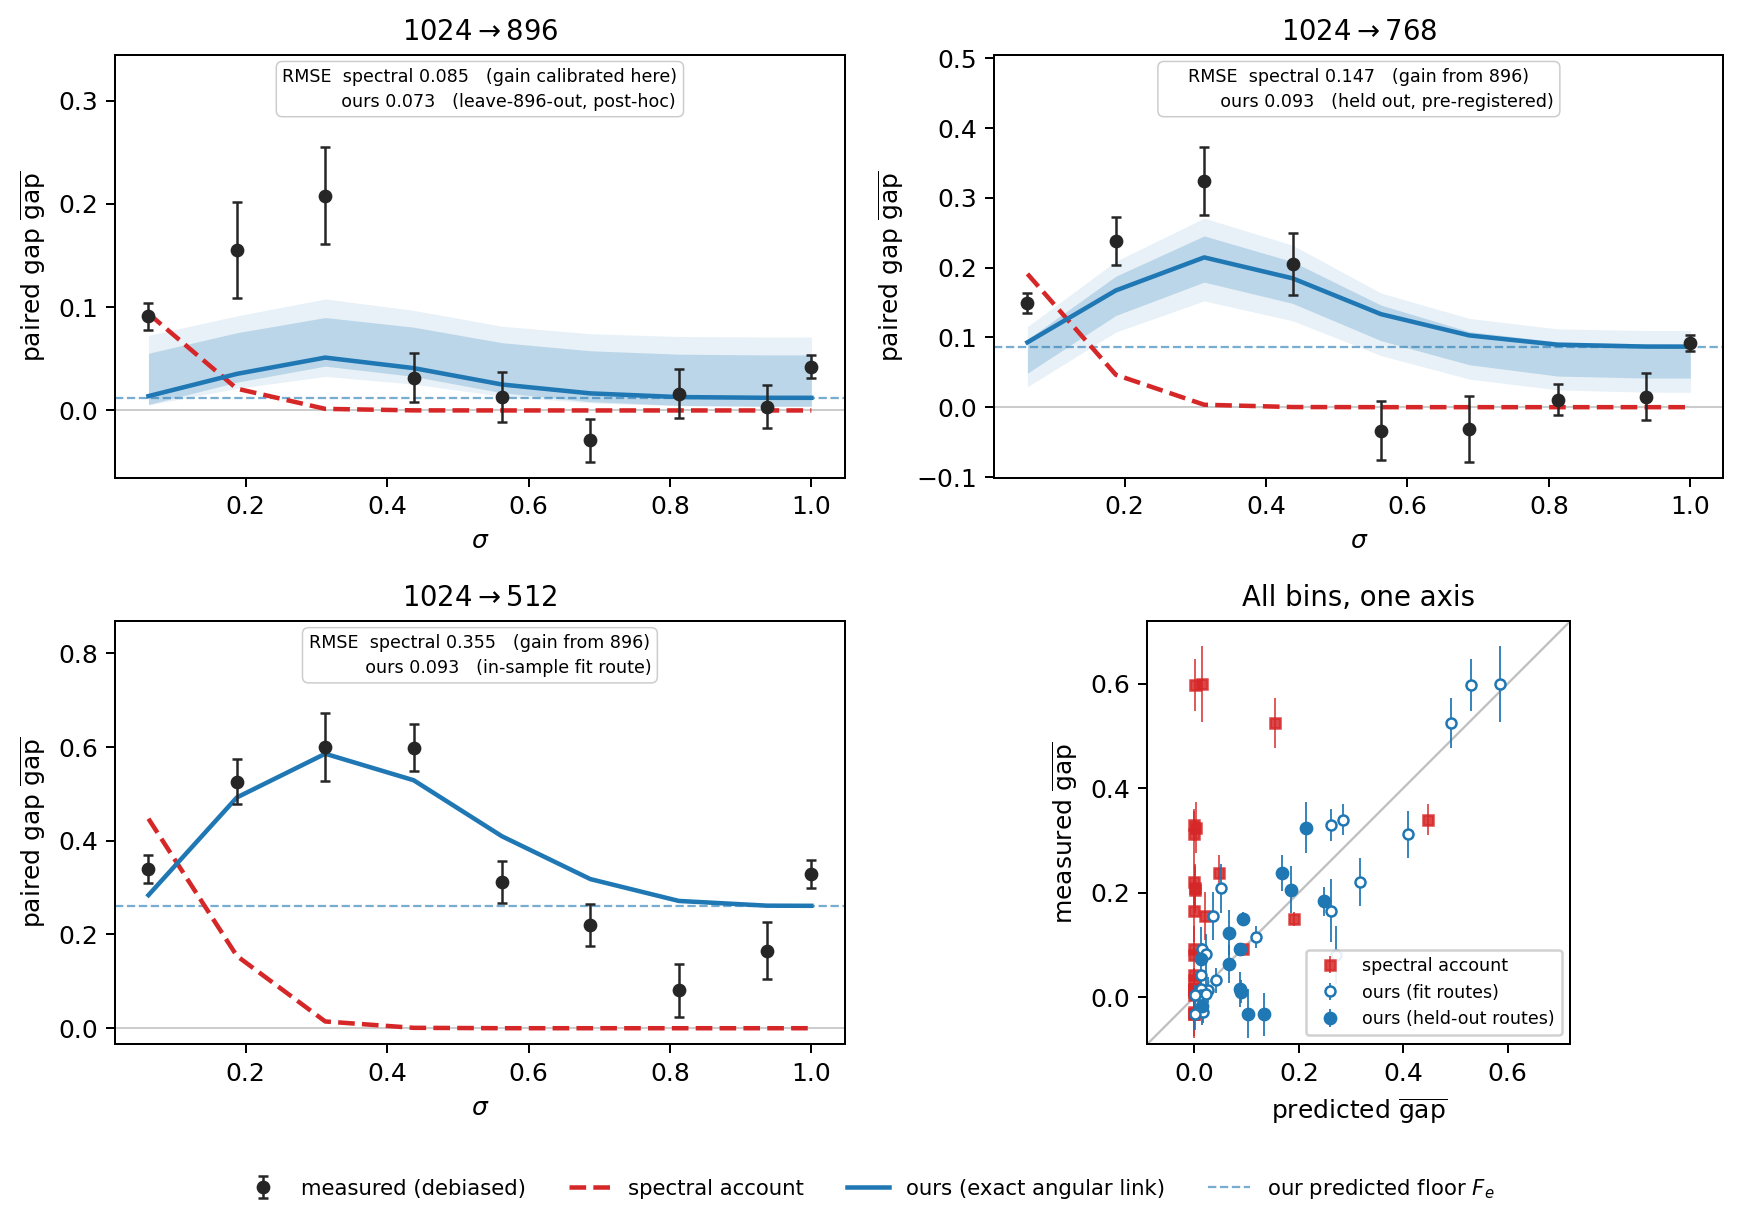
\includegraphics[width=\linewidth]{figs/accounts_headtohead.png}
\caption{\textbf{Both accounts on the same axes.} Per route, one set of
measured debiased gap curves (Eq.~\ref{eq:gapdef}, black) carries both
predictions of \S\ref{sec:theory}: the spectral account (red dashed;
transported through the residual$\to$gradient bridge at the measured
anchor tolerance --- the whole family scores alike, Appendix
Fig.~\ref{fig:e83}) and ours under the exact angular link (blue,
Eq.~\ref{eq:exact}; three-form comparison in Appendix
Fig.~\ref{fig:e51280}), with each route's predicted floor (blue dashed
--- dashed-to-solid is the data term) and a $68\%/95\%$ full-pipeline
bootstrap band ($B{=}1000$; Appendix~\ref{app:instrument}). Neither
account is fit to the route it is drawn on except as labelled
in-panel: ours predicts $1024{\to}768$ from governors alone with zero
per-route freedom (pre-registered held-out) and $1024{\to}896$ under
the post-hoc leave-$896$-out re-derivation, while the spectral
account's single gain is calibrated on $1024{\to}896$ and frozen. The
$768$ mid-$\sigma$ dip and the $896$ low-$\sigma$ plateau sit outside
the $95\%$ band --- the two edges of the reduction's domain
(Appendix~\ref{sec:headtohead}). Bottom right: predicted vs measured
over every bin, with ours also on the two $1280$-tier routes the
spectral bridge does not cover.}
\label{fig:accounts}
\end{figure}

Both accounts are scored against one measured object: the debiased gap
curves of Figs.~\ref{fig:accounts} and~\ref{fig:verdict}, whose per-bin
reading \S\ref{sec:map} has just set out. Four features of
those curves are all the scoring needs: the $896$ route enters the
re-encoding band at $\sigma \approx 0.5$, $768$ falls only to a low
but persistent excess at high noise (its $(0.65, 0.95)$ window),
$512$ is gapped at every noise level, and every route's
high-$\sigma$ plateau converges to a nonzero level ordered by the
target grid's token count. We score the spectral account against those
features first, at the boundary and then the curve level, and ours
after, term by term.

\paragraph{The spectral account: boundaries, curves, and an inert
$\delta$.}
The Qwen-Image VAE's latents are high-frequency-quiet ($P(f) < 1$ above
$f \approx 0.16$ cycles/latent-pixel; latent variance $0.42$), giving
equal-power crossovers of $0.136 / 0.146 / {\approx}\,0.20$ for
$896/768/512$: at that tolerance demotion would be safe over almost
the entire $\sigma$ axis.
Table~\ref{tab:null} (Appendix~\ref{app:spectral}) sweeps the whole
tolerance family, and no row reproduces the measured map
(\S\ref{sec:map}) --- including the zero-free-parameter member
anchored by our own pipeline's measured re-encode error, which lands
maximally conservative and is still structurally wrong in both
directions at once. At the curve level (Fig.~\ref{fig:e83}, the family
transported to full curves) the failure is sharper: the predicted
mismatch is concentrated below $\sigma \approx 0.3$ and the
transported curve is near zero exactly where the measured curves peak
(RMSE $0.147$ at $768$ and $0.355$ at $512$), while above each
tolerance's committed boundary, where every member predicts exactly
zero, the floor persists (committed-region RMSE $0.027/0.049/0.218$
for $896/768/512$). And because the transported curve has already died
by $\sigma \approx 0.35$, every tolerance scores within $0.01$ RMSE of
every other: $\delta$, the family's one degree of freedom, is
\emph{inert} at the curve level, so the structural failures of
\S\ref{sec:spectral}(a--c) do not hinge on its choice. Both reads are
insensitive to the residual-shape choice in the transport.


\paragraph{Ours, first term: the graph term exists (three probes, one
number).}
At the $\sigma = 1$ \emph{endpoint} the input is pure $\epsilon$,
identical in distribution across arms, so the input-mediated data term
is zero by construction; the debiased endpoint floors are
$+0.019 / +0.056 / +0.304$ for $896/768/512$ (Appendix
Table~\ref{tab:floor}),
and the $512$ value clears the pre-registered confirmation bar
($\dgap_\infty \ge 0.15$) on $12$ of $12$ probe images individually.
Per \S\ref{sec:ouraccount} the target-mediated share need not vanish
there, so two further probes close the step. The \emph{x-zero} probe
removes the image from input \emph{and} target everywhere, isolating
pure graph-shape sensitivity, and its debiased draw-limit gaps equal
the endpoint gaps at every route. The \emph{target-strength sweep}
re-runs the endpoint with target $\epsilon - \alpha x$,
$\alpha \in \{0, \ldots, 1\}$, and the paired debiased excess is
$\alpha$-flat at the well-conditioned anchors (e.g.\ $768$:
$+0.070 \pm 0.015$ at $\alpha{=}0$ vs $+0.049 \pm 0.010$ at
$\alpha{=}1$; control slope $+0.003$): no resolvable target-content
share \emph{in the angular estimand}. The flatness is not a
cancellation mystery: the target-mediated gradient itself is real and
large, but demotion's change to it lands almost entirely \emph{along}
$\hat g_{\src}$, to which the cosine gap is blind (Eq.~\ref{eq:exact})
--- the endpoint gap is the graph floor as the angular estimand reads
it (parallel-landing decomposition, with the
$\kappa_\parallel/\kappa_\perp$ numbers, in
Appendix~\ref{app:instrument}). Finally, a forward-only probe of the
model's caption-conditioned \emph{prior} across grids gives route
distances that are flat where the floors are strongly ordered, placing
the ordering in $J$ rather than in a resolution-conditioned prior or a
training-distribution discontinuity.

\paragraph{The data branch: a route-uniform numerator over a U-shaped
denominator.}
Measuring the mean prediction residual
$\bar r = \mathbb{E}_\epsilon[\hat v - (\epsilon - x)]$ per grid and
$\sigma$ (the exact $r$ in $g = J^{\!\top}r$; by
Eq.~\ref{eq:appsplit} intrinsic posterior bias plus the frozen
model's approximation error, not model error alone) shows a strong, monotone
$\sigma$-shape (cross-grid excess $0.89 \to 0.36$ in relative $L_2$
from $\sigma{=}0.125$ to $1$) that is the \emph{same for every route}
within $\pm 0.02$, across routes whose gradient floors span $0$ to
$0.3$ (Appendix Table~\ref{tab:residual}). This kills the
residual-level prediction of \S\ref{sec:spectral}: with no
cross-frequency coupling, that mismatch is confined to the destroyed
band and ordered by its energy, which differs substantially across
these routes. Route-uniformity says the real mismatch is carried by
cross-band structure the diagonal model cannot express, and that all
route identity lives in $J$ --- a pre-registered contrast that would
equally have falsified our own assumption~(iv); instead it
\emph{establishes} the shape factorization directly. The decay is
smooth, Wiener-like shrinkage with no hard gate at the spectral
crossover.

The denominator then does real work: the total gradient norm is
U-shaped in $\sigma$ ($2.6 \to 0.4$ at $\sigma\!\approx\!0.3 \to 9.3$;
Fig.~\ref{fig:estimator}) --- large at high $\sigma$ where the model
pulls composition out of the prior, small in the mid-$\sigma$
refinement regime, inflated again at low $\sigma$ by irreducible
$\epsilon$. A monotone absolute mismatch over a U-shaped norm yields
exactly the measured interior-peaked curves: bin-mean gap tracks
$1/\|\bar g_{\src}\|$ (Spearman $+0.55$--$+0.90$), and
renormalizing by $\|\bar g_{\src}\|$ flips the
anomalous low-$\sigma$ dip into the monotone maximum in every arm of
both runs. This is a post-hoc consistency analysis (so labeled): it
explains the \emph{shape}; all safety criteria stay in cosine units,
since direction is what a normalized optimizer consumes.

\paragraph{The governors: ratio sets the amplitude, absolute size sets
the floor.}
With the floor isolated, what orders the routes? Two probes give a
clean division of labor, and together they decide the equal-ratio
disagreement --- limit~(b) of \S\ref{sec:spectral}. \emph{Absolute
size, not ratio, sets the floor}: re-run one tier down, the route
$896{\to}768$ fails its pre-registered bar with a high-$\sigma$
residual ${\sim}2\times$ the $1024{\to}896$ plateau despite a
near-identical downscale ratio, while the two routes sharing the
${\sim}2{,}160$-token target grid, $1024{\to}768$ and $896{\to}768$,
land on the same floor despite different ratios (Appendix
Table~\ref{tab:phase1a}). Near-equal ratio, different target:
different verdict; same target, different ratio: same floor ---
refuting any pure ratio rule for the floor, and with it the spectral
account's only degree of freedom. And the floor grows monotonically as
the \emph{target} grid shrinks ($0.02$--$0.04$ / $0.06$--$0.09$ /
${\approx}\,0.30$ at target ${\sim}3{,}000/2{,}160/1{,}000$ tokens),
consistent with ``floor $=$ how well the coarse graph approximates the
fine graph's computation.''
\emph{Ratio, not absolute size, sets the amplitude}: a synthetic
iso-severity route $1280{\to}1120$ (edge ratio exactly matched to
$1024{\to}896$, at $1.6\times$ its absolute target size) reproduces
the $1024{\to}896$ curve bin-for-bin, crossover included (Appendix
Table~\ref{tab:isoseverity}). Note what survives of
the spectral account here: ratio \emph{is} the right governor for the
data term; its error is not its governor but its scope, mistaking one
term for the whole gap.

\paragraph{The floor's own parts: $\Floor_e = \mathrm{RoPE}_e +
\mathrm{Resid}_e$.}
The prediction of \S\ref{sec:reduction} --- that the positional share
is a coordinate-system artifact --- is testable by an origin-side
intervention: evaluate the demoted grid at positionally-interpolated
fractional rotary coordinates (patch $i$ at $i \cdot
H_{\src}/H_{\dem}$), making its relative phase geometry exactly match
native. At the $\sigma{=}1$ endpoint this \emph{erases} the $768$ floor
and removes ${\sim}30\%$ of the $512$ floor, leaving the
in-band $896$ control untouched: re-anchored against the debiased
floors, $\mathrm{Resid}_{768} \approx 0$ while $512$ retains a
$\mathrm{Resid}_{512} \approx 0.2$ bulk. The mild-route floor is mostly
a coordinate-system artifact; the harsh-route bulk is a genuine
non-positional graph residue, and the capacity governor attaches to it,
as the band-counting sketch anticipated. The erasure is \emph{not} a
training lever --- with image content in the input the stretched
forward is off-manifold --- but a frequency-\emph{selective} banded
alignment survives in-window (\S\ref{sec:trainer}). Full numbers, the
per-block/per-module depth localization behind this design, and the
inference-side prior art on the attention-over-$N$ piece
\citep{li2025infoscale,liu2026tide} are in
Appendix~\ref{app:instrument}.

